\documentclass[12pt, titlepage]{article}

\usepackage{fullpage}
\usepackage[round]{natbib}
\usepackage{multirow}
\usepackage{booktabs}
\usepackage{tabularx}
\usepackage{graphicx}
\usepackage{float}
\usepackage{hyperref}
\hypersetup{
    colorlinks,
    citecolor=black,
    filecolor=black,
    linkcolor=red,
    urlcolor=blue
}
\usepackage[round]{natbib}

\newcounter{acnum}
\newcommand{\actheacnum}{AC\theacnum}
\newcommand{\acref}[1]{AC\ref{#1}}

\newcounter{ucnum}
\newcommand{\uctheucnum}{UC\theucnum}
\newcommand{\uref}[1]{UC\ref{#1}}

\newcounter{mnum}
\newcommand{\mthemnum}{M\themnum}
\newcommand{\mref}[1]{M\ref{#1}}

\title{SE 3XA3: Module Guide\\Tetris Tussle}

\author{Nicholas Lobo \\ lobon3 \\ 400179304 \and
	Matthew Paulin \\ paulinm \\ 400187147 \and
	David Carrie \\ carriedd \\ 000661652 \and
}

\date{\today}



\begin{document}

\maketitle

\pagenumbering{roman}
\tableofcontents
\listoftables
\listoffigures

\begin{table}[H]
\caption{\bf Revision History}
\begin{tabularx}{\textwidth}{p{3cm}p{2cm}X}
\toprule {\bf Date} & {\bf Version} & {\bf Notes}\\
\midrule
16/03/2021 & 1.0 & Finished sections 1 and 7\\
17/03/2021 & 1.1 & Finished sections 2, 3, and 4\\
18/03/2021 & 2.0 & Completed MG\\
\bottomrule
\end{tabularx}
\end{table}

\newpage

\pagenumbering{arabic}

\section{Introduction}
\subsection{Overview}
 Tetris took the world by storm in the 1980’s becoming the first hit game ever created by selling over 202 million copies. The aim of the development of Tetris Tussle is to take a bare bones version of this game and update it to better suit the modern standards of gaming through updated visuals, extra features, and player versus player (PvP) interaction
\subsection{Context}
This document is the Module Guide (MG) and is based on the previously created Software Requirements Specification (SRS). The SRS contains information about the functional and non-functional requirements that will guide the creation of a correct system. The MG specifies the modular structure of the system and is intended to allow both designers and maintainers to easily identify the parts of the software. The potential readers of this document include new project members, maintainers of the software, and the project's designers. New project members can use this document to easily and quickly understand the overall structure of the software and well as find the modules relevant to them. Maintainers can use the hierarchical structure of the MG to guide their modifications to the system and update this document when changes are made. Lastly, designers can use the completed MG to check for consistency among modules, feasibility of the decomposition, and the design's flexibility. After this document, a Module Interface Specification (MIS) will be created to provide detailed information about each individual module.

\subsection{Design Principles}
The design principle that is being used to guide the design of the software system is information hiding. Information hiding is the principle that each module hides a design decision from the rest of the system. Through decomposition, based on this principle, the system can be designed for change. This is invaluable because during development, modifications are very frequent. The principle of information hiding is followed by separating likely changes as the secrets of their own modules. Additionally, each data structure is used in only one module and any other module that requires information stored in a module's data structure will obtain it by calling access programs belonging to that module. This principle also enables high cohesion, low coupling, and no cycles among modules. High Cohesion refers to elements of a module being closely related. This vastly increases the software's maintainability because related functionality will be localized to an area of the software. Low coupling states that modules not be reliant on other modules. Module independence ensures that changes can be made to one module without altering another. No cycles means that no two modules will use each other, thus making the code easier to understand and maintain. 

\subsection{Document Structure}
The rest of the document is organized as follows. Section
\textbf{\ref{SecChange}} lists the anticipated and unlikely changes of the software
requirements. Section \textbf{\ref{SecMH}} summarizes the module decomposition that
was constructed according to the likely changes. Section \textbf{\ref{SecConnection}}
specifies the connections between the software requirements and the
modules. Section \textbf{\ref{SecMD}} gives a detailed description of the
modules. Section \textbf{\ref{SecTM}} includes two traceability matrices. One checks
the completeness of the design against the requirements provided in the SRS. The
other shows the relation between anticipated changes and the modules. Section \textbf{\ref{SecUse}} describes the uses relation between modules

\section{Anticipated and Unlikely Changes} \label{SecChange}
This section lists possible changes to the system. According to the likeliness
of the change, the possible changes are classified into two
categories. Anticipated changes are listed in Section \ref{SecAchange}, and
unlikely changes are listed in Section \ref{SecUchange}.

\subsection{Anticipated Changes} \label{SecAchange}

%Anticipated changes are the source of the information that is to be hidden
%inside the modules. Ideally, changing one of the anticipated changes will only
%require changing the one module that hides the associated decision. The approach
%adapted here is called design for
%change.

\begin{description}
\item[\refstepcounter{acnum} \actheacnum \label{acHardware}:] The specific
  hardware on which the software is running.
\item[\refstepcounter{acnum} \actheacnum \label{acInput}:] The format of the
  initial input data.
\item[\refstepcounter{acnum} \actheacnum \label{acScore}:] The calculation of the score
\item[\refstepcounter{acnum} \actheacnum \label{acMenu}:] The design and format of the menu
\item[\refstepcounter{acnum} \actheacnum \label{acBoard}:] The board customization
\item[\refstepcounter{acnum} \actheacnum \label{acMulti}:] The amount of players in one multiplayer lobby
\item[\refstepcounter{acnum} \actheacnum \label{acCustomize}:] The Tetromino customization
\item[\refstepcounter{acnum} \actheacnum \label{acGameplay}:] The multiplayer gameplay 
\end{description}

\subsection{Unlikely Changes} \label{SecUchange}

\begin{description}
\item[\refstepcounter{ucnum} \uctheucnum \label{ucIO}:] Input/Output devices
  (Input: Keyboard, Output: Screen/Server).
\item[\refstepcounter{ucnum} \uctheucnum \label{ucInput}:] There will always be
  a source of input data external to the software.
\item[\refstepcounter{ucnum} \uctheucnum \label{ucTetris}:] The purpose and objective of Tetris
\item[\refstepcounter{ucnum} \uctheucnum \label{ucP5JS}:] The usage of the p5.js library for the implementation of the software
\item[\refstepcounter{ucnum} \uctheucnum \label{ucServer}:] The usage of a server for multiplayer functionality
\item[\refstepcounter{ucnum} \uctheucnum \label{ucSocket}:] The usage of a socket interaction for input output functionality  
\item[\refstepcounter{ucnum} \uctheucnum \label{ucDesign}:] The design pattern and architecture for the software 
\item[\refstepcounter{ucnum} \actheacnum \label{ucWebApp}:] The use of a web application to interact with the software
\end{description}

\section{Module Hierarchy} \label{SecMH}

This section provides an overview of the module design. Modules are summarized
in a hierarchy decomposed by secrets in Table \ref{TblMH}. The modules listed
below, which are leaves in the hierarchy tree, are the modules that will
actually be implemented.

\begin{description}
\item [\refstepcounter{mnum} \mthemnum \label{mBHH}:] Hardware Hiding Module: User Inputs Module
\item [\refstepcounter{mnum} \mthemnum \label{mBH}:] Behaviour Hiding Module: Main View Module
\item [\refstepcounter{mnum} \mthemnum \label{mBH1}:] Behaviour Hiding Module: Leaderboard Module
\item [\refstepcounter{mnum} \mthemnum \label{mBH2}:] Behaviour Hiding Module: Menu Module
\item [\refstepcounter{mnum} \mthemnum \label{mBH3}:] Behaviour Hiding Module: Singleplayer View Module
\item [\refstepcounter{mnum} \mthemnum \label{mBH4}:] Behaviour Hiding Module: Multiplayer View Module
\item [\refstepcounter{mnum} \mthemnum \label{mBH5}:] Behaviour Hiding Module: Singleplayer Module
\item [\refstepcounter{mnum} \mthemnum \label{mBH6}:] Behaviour Hiding Module: Multiplayer Module
\item [\refstepcounter{mnum} \mthemnum \label{mBH7}:] Behaviour Hiding Module: Player Module
\item [\refstepcounter{mnum} \mthemnum \label{mBH8}:] Behaviour Hiding Module: Tetromino Module
\item [\refstepcounter{mnum} \mthemnum \label{mBH9}:] Behaviour Hiding Module: Board Module
\item [\refstepcounter{mnum} \mthemnum \label{mSDH}:] Software Decision Hiding Module: Server Module
\end{description}


\begin{table}[H]
\centering
\begin{tabular}{p{0.3\textwidth} p{0.6\textwidth}}
\toprule
\textbf{Level 1} & \textbf{Level 2}\\
\midrule

{Hardware-Hiding Module}& N/A\\
\midrule

\multirow{7}{0.3\textwidth}{Behaviour-Hiding Module} 
& User Inputs Module\\
& Main View Module\\
& Leaderboard Module\\
& Menu Module\\
& Singleplayer View Module\\
& Multiplayer View Module\\
& Singleplayer Module\\
& Multiplayer Module\\
& Player Module\\
& Tetromino Module\\
& Board Module\\

\midrule

Software Decision Module & Server Module\\ 

\bottomrule

\end{tabular}
\caption{Module Hierarchy}
\label{TblMH}
\end{table}

\section{Connection Between Requirements and Design} \label{SecConnection}

The design of the system is intended to satisfy the requirements developed in
the SRS. In this stage, the system is decomposed into modules. The connection
between requirements and modules is listed in Table \ref{TblRT}.

\section{Module Decomposition} \label{SecMD}

Modules are decomposed according to the principle of ``information hiding''
proposed by \citet{ParnasEtAl1984}. The \emph{Secrets} field in a module
decomposition is a brief statement of the design decision hidden by the
module. The \emph{Services} field specifies \emph{what} the module will do
without documenting \emph{how} to do it. For each module, a suggestion for the
implementing software is given under the \emph{Implemented By} title. If the
entry is \emph{OS}, this means that the module is provided by the operating
system or by standard programming language libraries.  Also indicate if the
module will be implemented specifically for the software.

Only the leaf modules in the
hierarchy have to be implemented. If a dash (\emph{--}) is shown, this means
that the module is not a leaf and will not have to be implemented. Whether or
not this module is implemented depends on the programming language
selected.

\subsection{Hardware Hiding Modules (\mref{mBHH})}

\begin{description}
\item[Secrets:]The data structure and algorithm used to implement the virtual
  hardware.
\item[Services:]Serves as a virtual hardware used by the rest of the
  system. This module provides the interface between the hardware and the
  software. So, the system can use it to display outputs or to accept inputs.
\item[Implemented By:] OS, JavaScript
\end{description}

\subsection{Behaviour-Hiding Module}

\begin{description}
\item[Secrets:]The contents of the required behaviours.
\item[Services:]Includes programs that provide externally visible behaviour of
  the system as specified in the software requirements specification (SRS)
  documents. This module serves as a communication layer between the
  hardware-hiding module and the software decision module. The programs in this
  module will need to change if there are changes in the SRS.
\item[Implemented By:] HTML, CSS, JavaScript (p5.js, Node.js)
\end{description}
%%%%%%%%%%%%%%%%%%%%%%%%%%%%%%%%%%%%%%%%%%%%%%%%%%%%%%%%%%%%%%%%%%%%%%%
\subsubsection{User Inputs Module (\mref{mBHH})}
\begin{description}
\item[Secrets:]Inputs
\item[Services:]Converts the input data into the data structure used by the
  input parameters module.
\item[Implemented By:] JavaScript
\end{description}

\subsubsection{Main View Module (\mref{mBH})}
\begin{description}
\item[Secrets:]Graphics
\item[Services:]Draws the main screen.
\item[Implemented By:] JavaScript (p5.js)
\end{description}

\subsubsection{Leaderboard Module(\mref{mBH1})}
\begin{description}
\item[Secrets:] Score
\item[Services:] Displays point totals from the top scoring games.
\item[Implemented By:] JavaScript (p5.js)
\end{description}

\subsubsection{Menu Module (\mref{mBH2})}
\begin{description}
\item[Secrets:]Graphics
\item[Services:] Enables application navigation.
\item[Implemented By:] JavaScript (p5.js)
\end{description}

\subsubsection{Singleplayer View (\mref{mBH3})}
\begin{description}
\item[Secrets:]Graphics
\item[Services:]Draws the single player view representing the current state of a single player game of Tetris.
\item[Implemented By:] JavaScript (p5.js)
\end{description}

\subsubsection{Multiplayer View Module (\mref{mBH4})}
\begin{description}
\item[Secrets:]Graphics
\item[Services:]Draws the multiplayer view including a representation of a game of player versus player Tetris.
\item[Implemented By:] JavaScript (p5.js)
\end{description}

\subsubsection{Singleplayer Module (\mref{mBH5})}
\begin{description}
\item[Secrets:]Data
\item[Services:] Uses input data to store and manipulate the state of a singleplayer game of Tetris.
\item[Implemented By:] JavaScript (Node.js)
\end{description}

\subsubsection{Multiplayer Module(\mref{mBH6})}
\begin{description}
\item[Secrets:]Data
\item[Services:]Uses input data to store and manipulate the state of a multiplayer game of Tetris.
\item[Implemented By:] JavaScript (Node.js)
\end{description}

\subsubsection{Player Module (\mref{mBH7})}
\begin{description}
\item[Secrets:]Data
\item[Services:]Stores and shares information of the player state.
\item[Implemented By:] JavaScript (Node.js)
\end{description}

\subsubsection{Tetromino Module (\mref{mBH8})}
\begin{description}
\item[Secrets:]Data
\item[Services:]Stores and shares information of the Tetromino state.
\item[Implemented By:] JavaScript (Node.js)
\end{description}

\subsubsection{Board Module (\mref{mBH9})}
\begin{description}
\item[Secrets:]Data
\item[Services:]Stores and shares information of the board state.
\item[Implemented By:] JavaScript (Node.js)
\end{description}


%%%%%%%%%%%%%%%%%%%%%%%%%%%%%%%%%%%%%%%%%%%%%%%%%%%%%%%%%%%%%%%%%%%%%%%%%

\subsection{Software Decision Module}
\begin{description}
\item[Secrets:] The design decision based on mathematical theorems, physical
  facts, or programming considerations. The secrets of this module are
  \emph{not} described in the SRS.
\item[Services:] Includes data structure and algorithms used in the system that
  do not provide direct interaction with the user. 
  % Changes in these modules are more likely to be motivated by a desire to
  % improve performance than by externally imposed changes.
\item[Implemented By:] JavaScript (SocketIO, Node.js)
\end{description}

\subsubsection{Server Module (\mref{mSDH})}

\begin{description}
\item[Secrets:] Inter-module communication
\item[Services:] Facilitates communication between the clients and the server.
\item[Implemented By:] JavaScript (SocketIO, Node.js)
\end{description}

\section{Traceability Matrix} \label{SecTM}

This section shows two traceability matrices: between the modules and the
requirements and between the modules and the anticipated changes.

% the table should use mref, the requirements should be named, use something
% like fref
\begin{table}[H]
\centering
\begin{tabular}{p{0.2\textwidth} p{0.6\textwidth}}
\toprule
\textbf{Req.} & \textbf{Modules}\\
\midrule
BE1-FR1 &  \mref{mBHH}, \mref{mBH7}, \mref{mBH8}\\
BE1-FR2 & \mref{mBH7}, \mref{mBH8}\\
BE1-FR3 &  \mref{mBH7}, \mref{mBH8}\\
BE2-FR1 & \mref{mBHH},\mref{mBH7}\\
BE2-FR2 & \mref{mBHH},\mref{mBH7}\\
BE2-FR3 & \mref{mBHH},\mref{mBH7}\\
BE2-FR4 & \mref{mBHH},\mref{mBH7}\\
BE2-FR5 & \mref{mBH9}\\
BE2-FR6 & \mref{mBH7}, \mref{mBH8}\\
BE2-FR7 & \mref{mBH9}\\
BE2-FR8 & \mref{mBH9} \\
BE2-FR9 & \mref{mBH5}, \mref{mBH6} \\
BE2-FR10 & \mref{mBH5}, \mref{mBH6} \\
BE3-FR1 & \mref{mBH2}, \mref{mSDH}\\
BE3-FR2 & \mref{mBH2}, \mref{mSDH} \\
BE3-FR3 & \mref{mBH2}, \mref{mSDH} \\
BE3-FR4 & \mref{mBH} \\
BE3-FR5 & \mref{mBH8} \\
BE3-FR6 & \mref{mBH8} \\
BE3-FR7 & \mref{mBH5}, \mref{mBH6}\\
BE3-FR8 & \mref{mBH3}, \mref{mBH4} \\
BE3-FR9 &  \mref{mBH5}, \mref{mBH6}, \mref{mBH9} \\
BE4-FR1 & \mref{mBH1}\\
BE4-FR2 & \mref{mBH}\\
BE4-FR3 & \mref{mBH1}\\
BE4-FR4 & \mref{mBH1}\\
BE5-FR1 & \mref{mBH6}\\
BE5-FR2 & \mref{mBH6}\\
BE5-FR3 & \mref{mBH6}\\
BE6-FR1 & \mref{mBH6}\\
BE6-FR2 & \mref{mBH2},\mref{mBH6}\\
BE6-FR3 & \mref{mBH6}\\\\
\bottomrule
\end{tabular}
\caption{Trace Between Requirements and Modules}
\label{TblRT}
\end{table}

\begin{table}[H]
\centering
\begin{tabular}{p{0.2\textwidth} p{0.6\textwidth}}
\toprule
\textbf{AC} & \textbf{Modules}\\
\midrule
\acref{acHardware} & \mref{mBHH}\\
\acref{acInput} & \mref{mBHH}\\
\acref{acScore} & \mref{mSDH}\\
\acref{acMenu} & \mref{mBH}, \mref{mBH2}\\
\acref{acBoard} & \mref{mBH9}\\
\acref{acMulti} & \mref{mBH4}, \mref{mBH6}\\
\acref{acCustomize} & \mref{mBH8}\\
\acref{acGameplay} & \mref{mSDH}\\

\bottomrule
\end{tabular}
\caption{Trace Between Anticipated Changes and Modules}
\label{TblACT}
\end{table}

\section{Use Hierarchy Between Modules} \label{SecUse}

In this section, the uses hierarchy between modules is
provided. \citet{Parnas1978} said of two programs A and B that A {\em uses} B if
correct execution of B may be necessary for A to complete the task described in
its specification. That is, A {\em uses} B if there exist situations in which
the correct functioning of A depends upon the availability of a correct
implementation of B.  Figure \ref{FigUH} illustrates the use relation between
the modules. It can be seen that the graph is a directed acyclic graph
(DAG). Each level of the hierarchy offers a testable and usable subset of the
system, and modules in the higher level of the hierarchy are essentially simpler
because they use modules from the lower levels.

\begin{figure}[H]
\centering
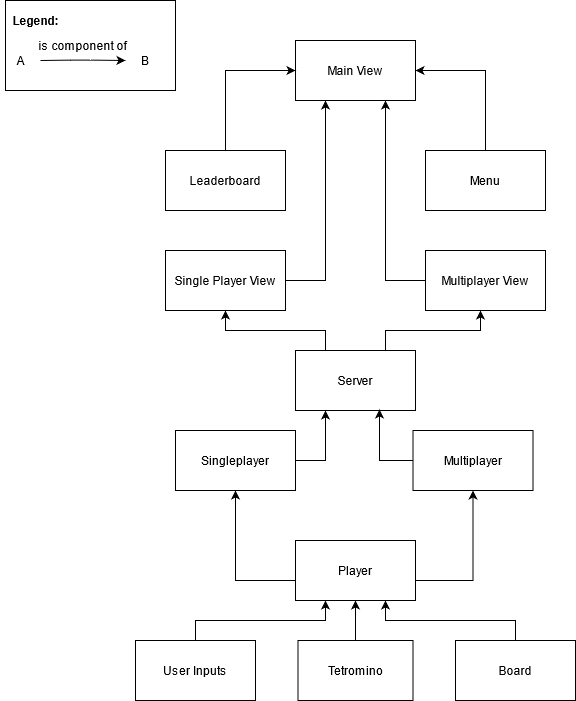
\includegraphics[width=1\textwidth]{MG/diagram.png} 

\caption{Use hierarchy among modules}
\label{FigUH}
\end{figure}

%\section*{References}

\bibliographystyle {plainnat}
\bibliography {MG/MG}

\end{document}